\documentclass{beamer}\usepackage[]{graphicx}\usepackage[]{xcolor}
% maxwidth is the original width if it is less than linewidth
% otherwise use linewidth (to make sure the graphics do not exceed the margin)
\makeatletter
\def\maxwidth{ %
  \ifdim\Gin@nat@width>\linewidth
    \linewidth
  \else
    \Gin@nat@width
  \fi
}
\makeatother

\definecolor{fgcolor}{rgb}{0.345, 0.345, 0.345}
\newcommand{\hlnum}[1]{\textcolor[rgb]{0.686,0.059,0.569}{#1}}%
\newcommand{\hlsng}[1]{\textcolor[rgb]{0.192,0.494,0.8}{#1}}%
\newcommand{\hlcom}[1]{\textcolor[rgb]{0.678,0.584,0.686}{\textit{#1}}}%
\newcommand{\hlopt}[1]{\textcolor[rgb]{0,0,0}{#1}}%
\newcommand{\hldef}[1]{\textcolor[rgb]{0.345,0.345,0.345}{#1}}%
\newcommand{\hlkwa}[1]{\textcolor[rgb]{0.161,0.373,0.58}{\textbf{#1}}}%
\newcommand{\hlkwb}[1]{\textcolor[rgb]{0.69,0.353,0.396}{#1}}%
\newcommand{\hlkwc}[1]{\textcolor[rgb]{0.333,0.667,0.333}{#1}}%
\newcommand{\hlkwd}[1]{\textcolor[rgb]{0.737,0.353,0.396}{\textbf{#1}}}%
\let\hlipl\hlkwb

\usepackage{framed}
\makeatletter
\newenvironment{kframe}{%
 \def\at@end@of@kframe{}%
 \ifinner\ifhmode%
  \def\at@end@of@kframe{\end{minipage}}%
  \begin{minipage}{\columnwidth}%
 \fi\fi%
 \def\FrameCommand##1{\hskip\@totalleftmargin \hskip-\fboxsep
 \colorbox{shadecolor}{##1}\hskip-\fboxsep
     % There is no \\@totalrightmargin, so:
     \hskip-\linewidth \hskip-\@totalleftmargin \hskip\columnwidth}%
 \MakeFramed {\advance\hsize-\width
   \@totalleftmargin\z@ \linewidth\hsize
   \@setminipage}}%
 {\par\unskip\endMakeFramed%
 \at@end@of@kframe}
\makeatother

\definecolor{shadecolor}{rgb}{.97, .97, .97}
\definecolor{messagecolor}{rgb}{0, 0, 0}
\definecolor{warningcolor}{rgb}{1, 0, 1}
\definecolor{errorcolor}{rgb}{1, 0, 0}
\newenvironment{knitrout}{}{} % an empty environment to be redefined in TeX

\usepackage{alltt}
\usepackage{graphicx}
\usepackage{booktabs}

\title{Presentación de Análisis de Datos}
\author{Ana G. Dos Santos F.}
\date{2024-07-24}
\usetheme{Berlin}
\IfFileExists{upquote.sty}{\usepackage{upquote}}{}
\begin{document}

\begin{frame}
  \titlepage
\end{frame}

\begin{frame}
  \frametitle{Índice}
  \tableofcontents
\end{frame}

\section{Introducción}
\begin{frame}
  \frametitle{Introducción}
  Este informe presenta el análisis de los datos depurados del conjunto de datos ESS9e03\_2-ESS10.
\end{frame}

\section{Gráficos Principales}
\begin{frame}
  \frametitle{Gráficos Principales}
  A continuación, se muestran los principales gráficos obtenidos del análisis de datos.
\end{frame}



\begin{frame}
\frametitle{Gráfico}
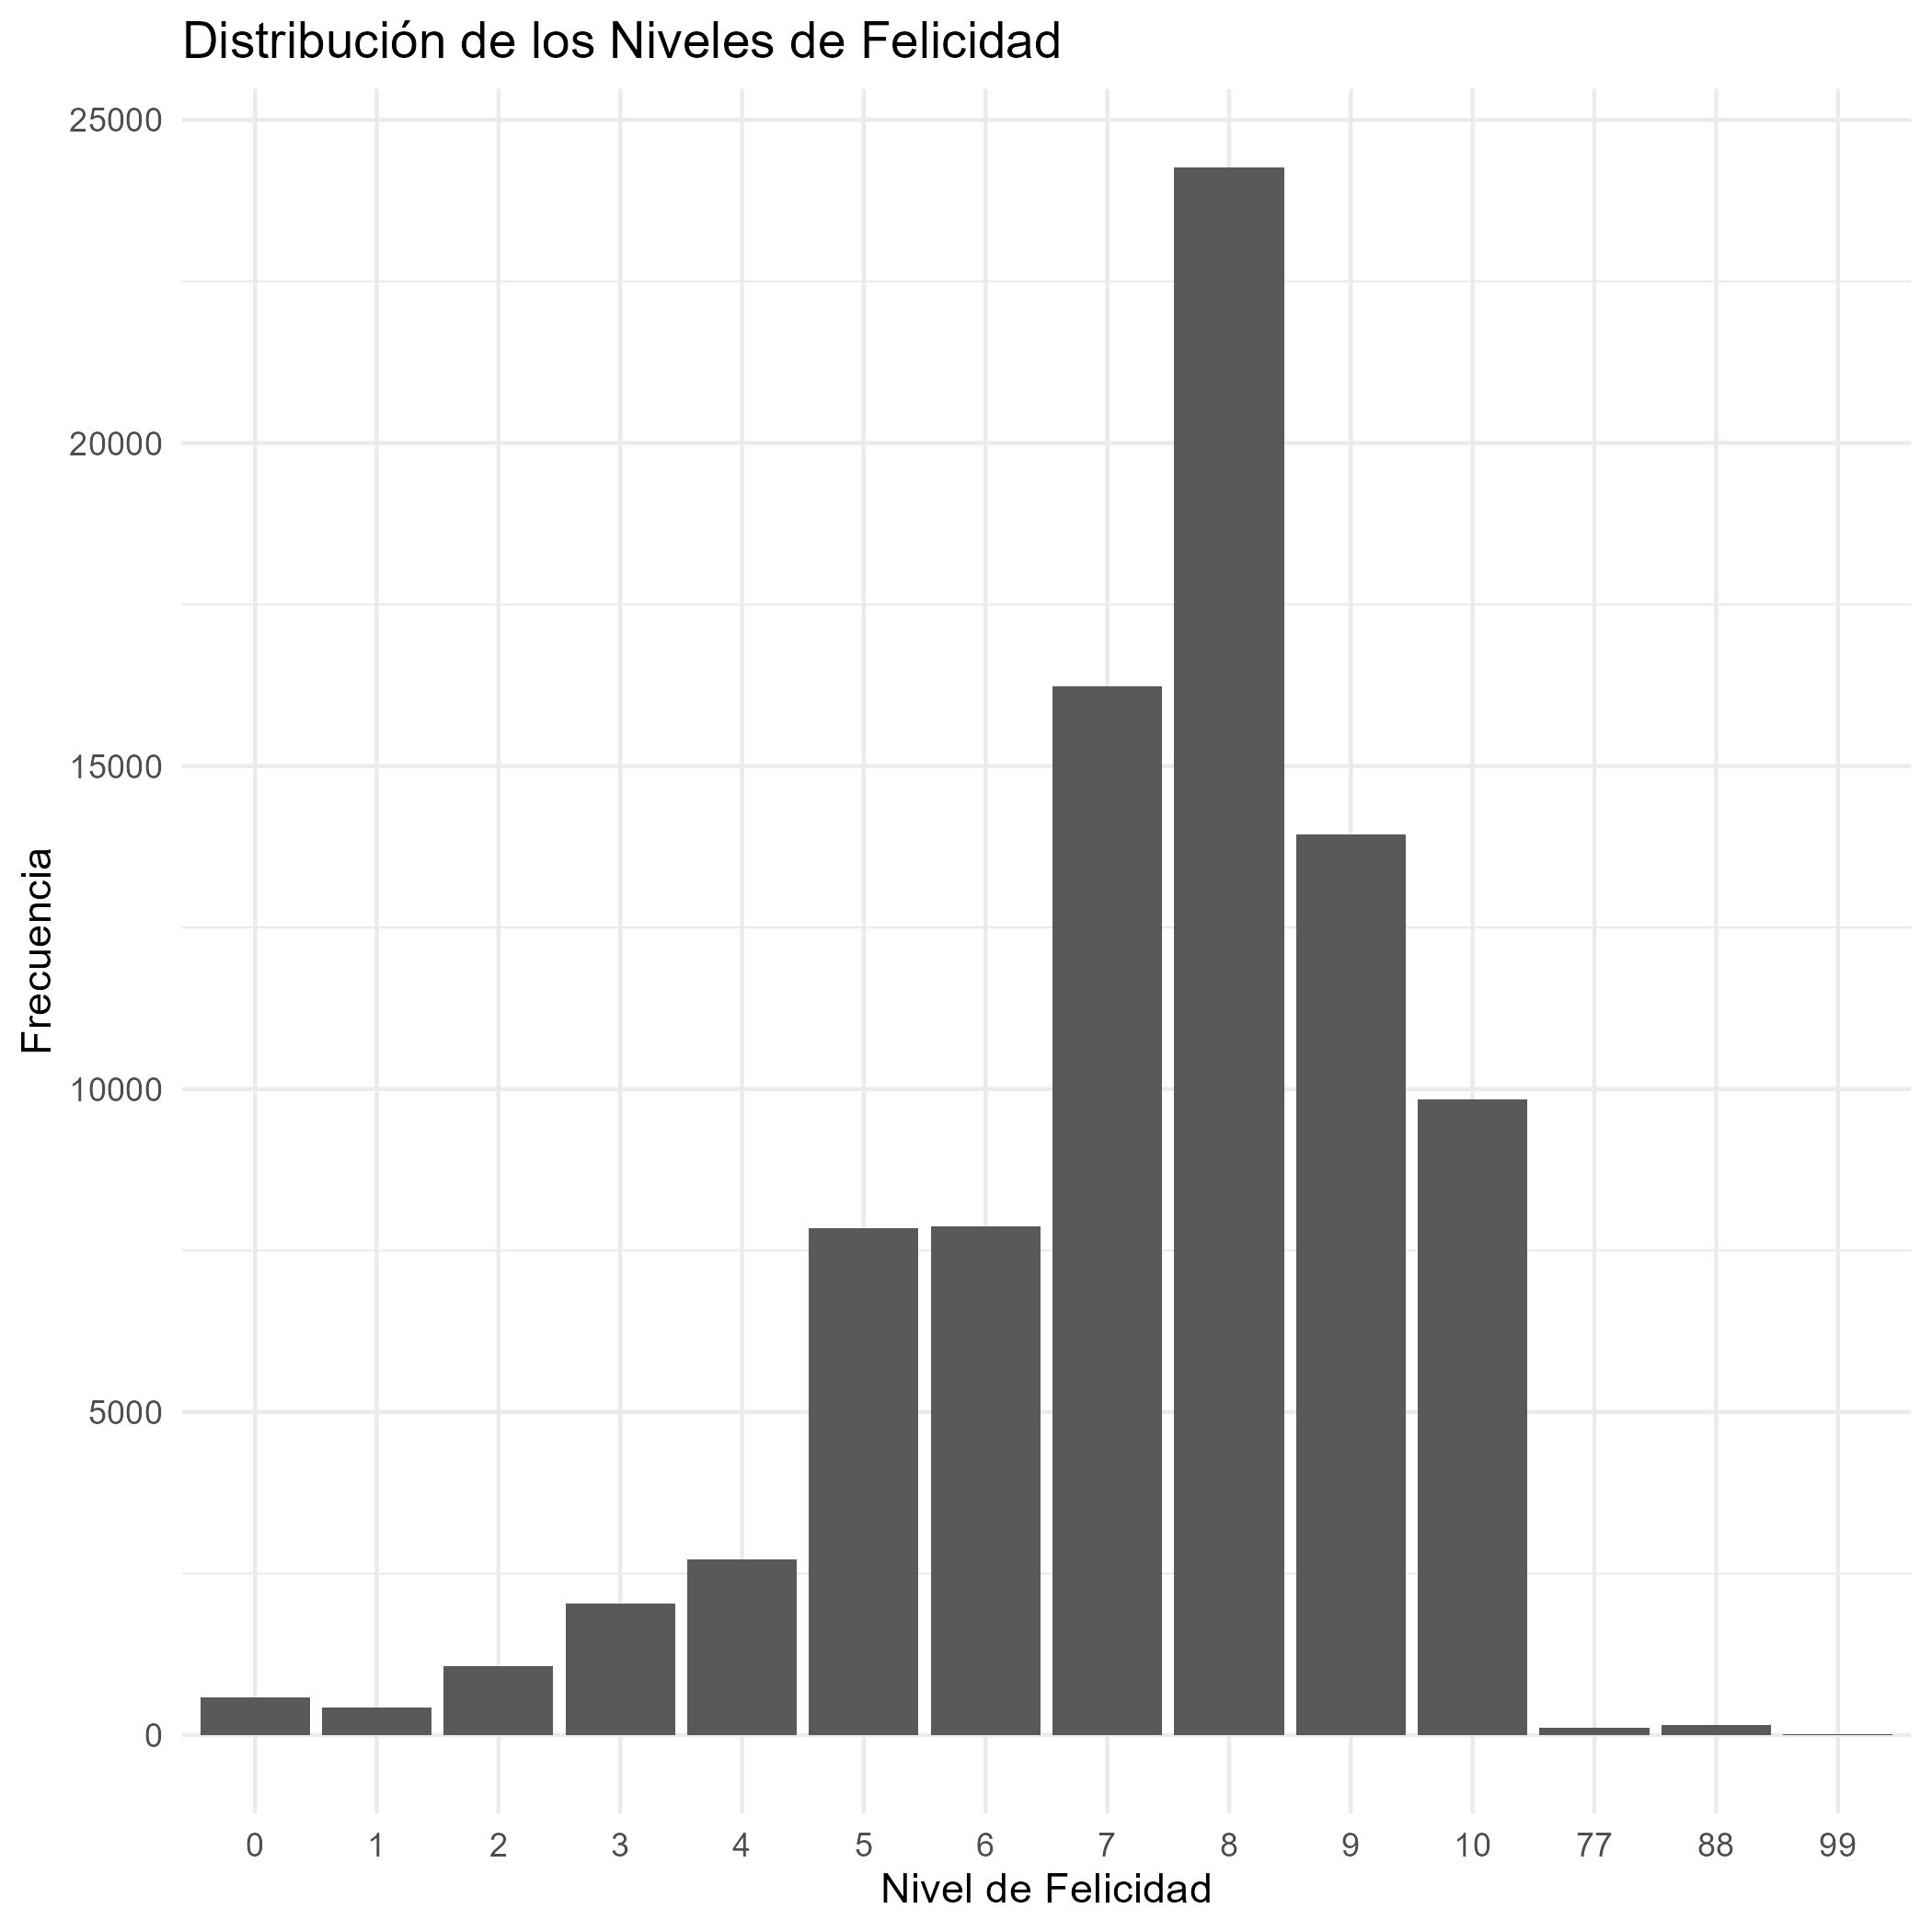
\includegraphics[width=0.8\textwidth]{C:/Users/User/Desktop/GITHUB/ProyectoCD---Modulo-8-Julio2024/INFORME/distribucion_felicidad.png}
\end{frame}
\begin{frame}
\frametitle{Gráfico}
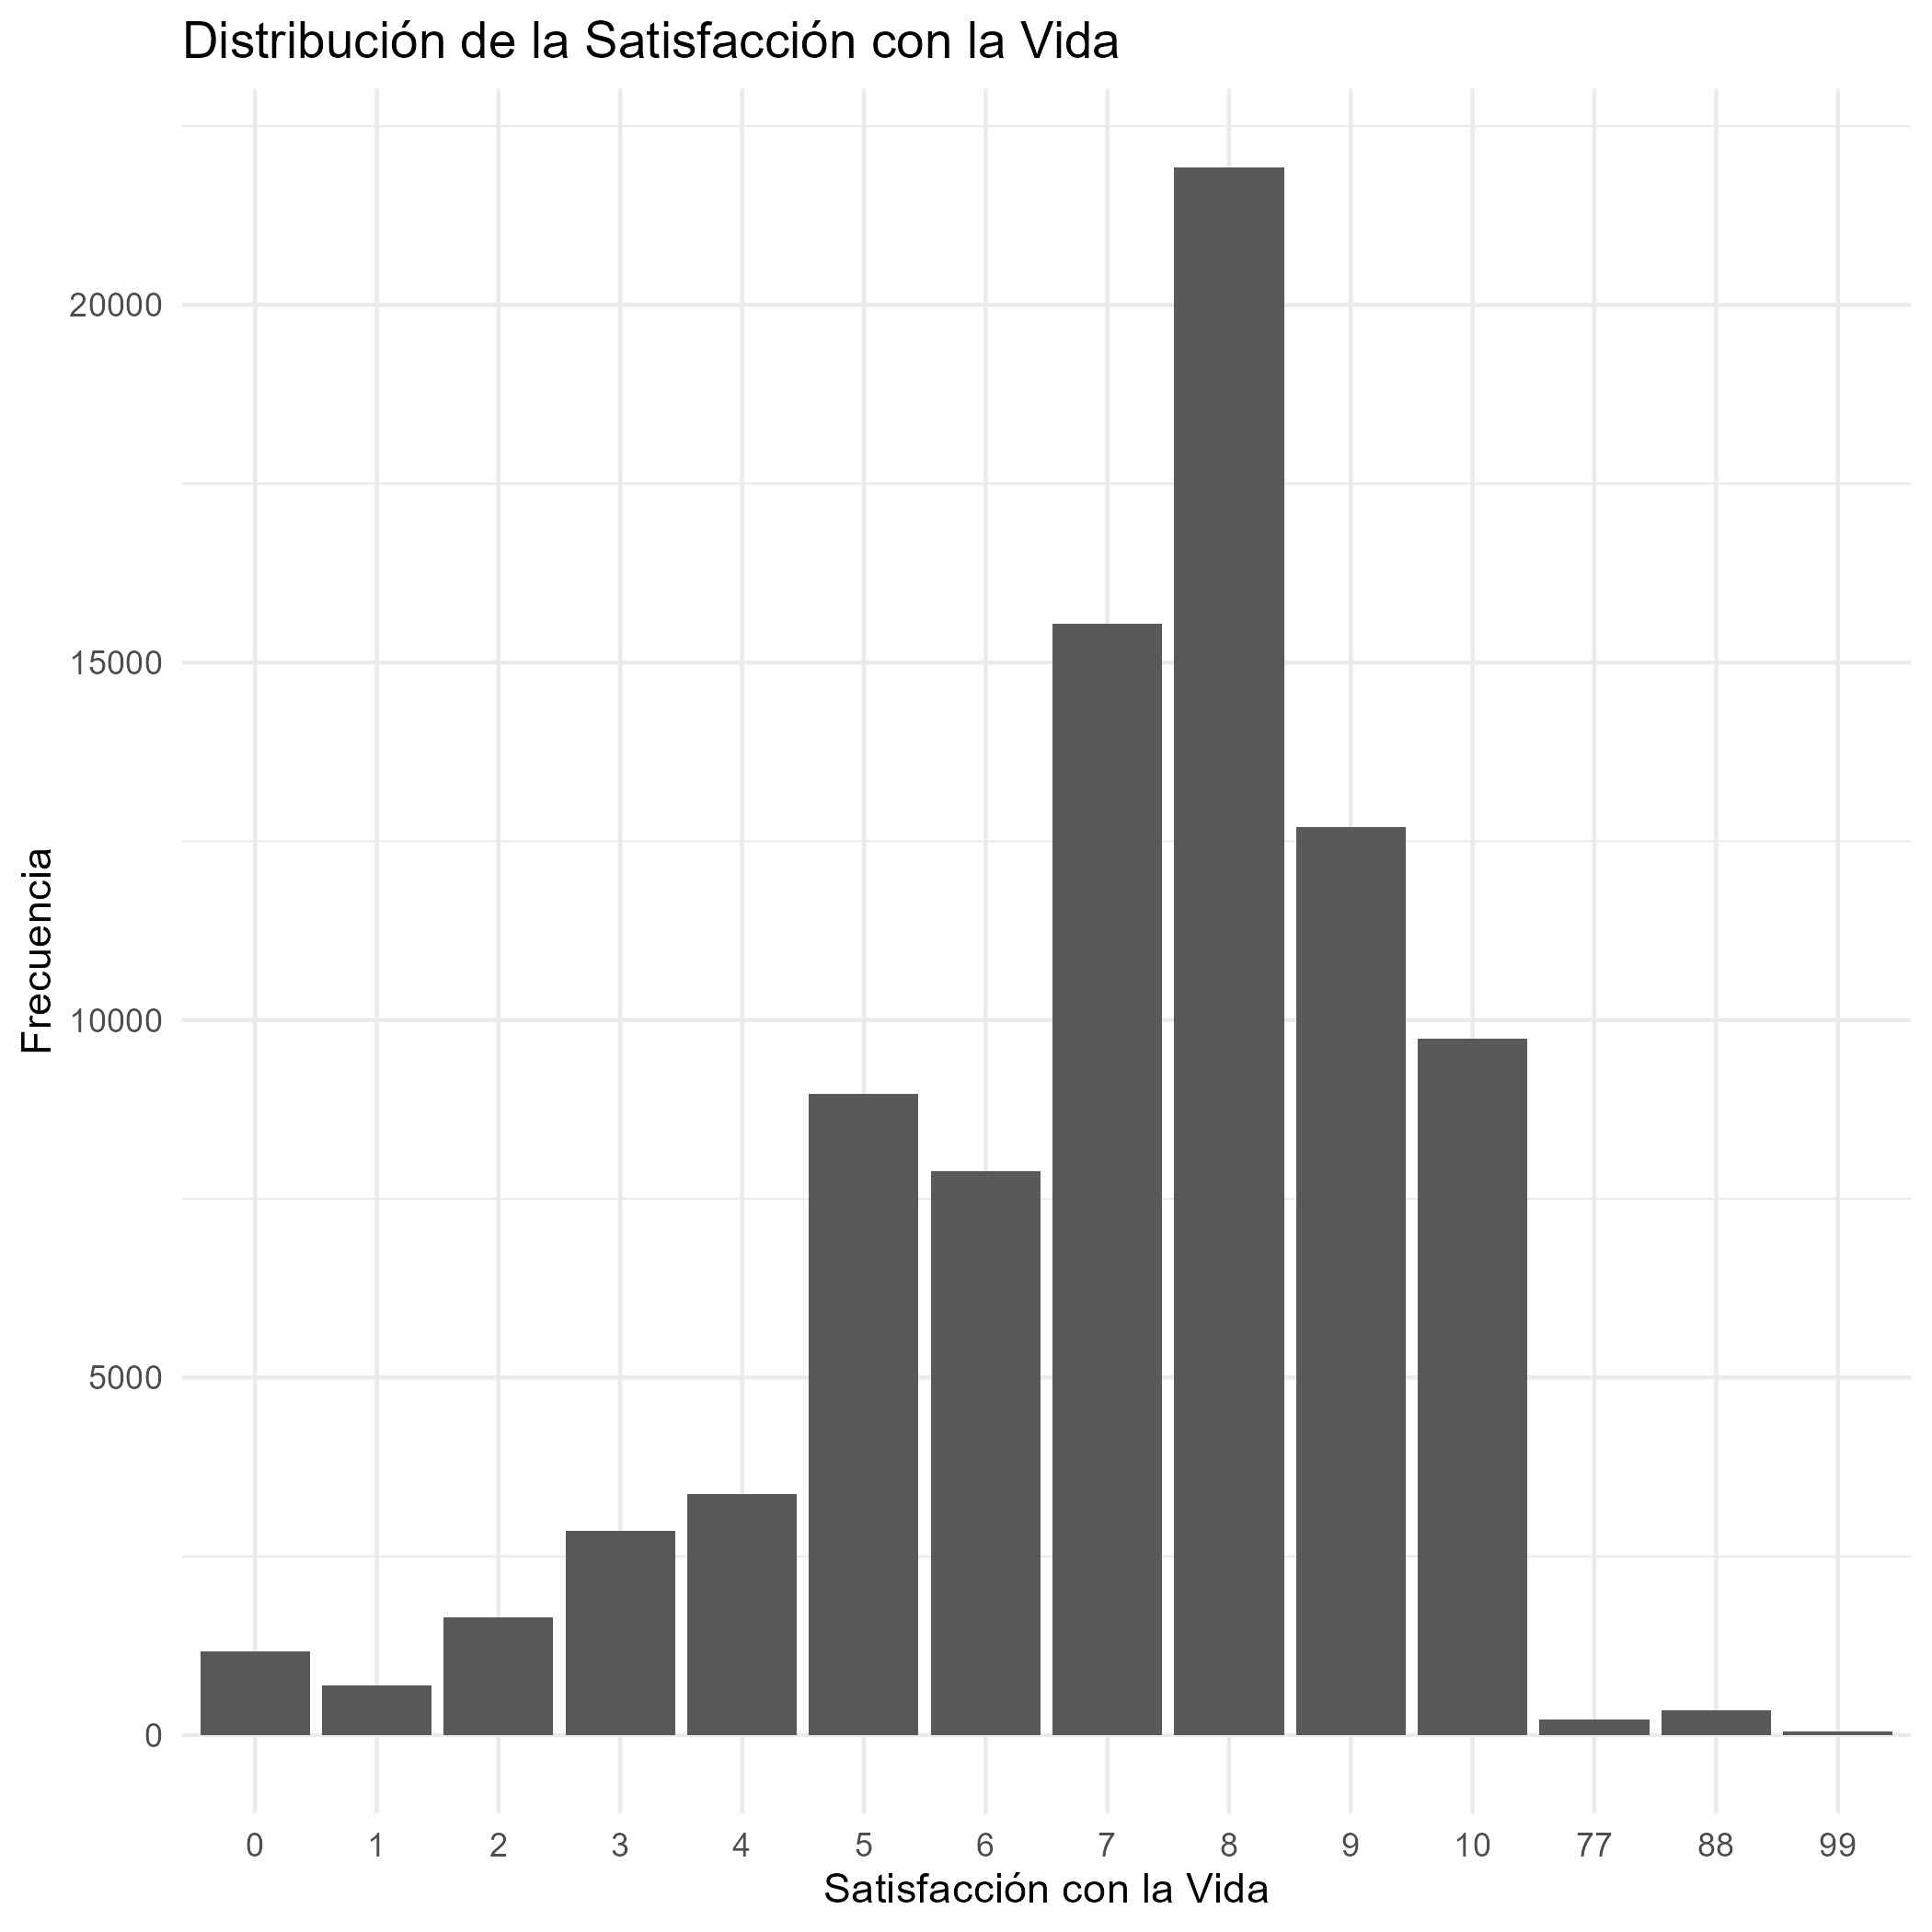
\includegraphics[width=0.8\textwidth]{C:/Users/User/Desktop/GITHUB/ProyectoCD---Modulo-8-Julio2024/INFORME/distribucion_satisfaccion_vida.png}
\end{frame}
\begin{frame}
\frametitle{Gráfico}
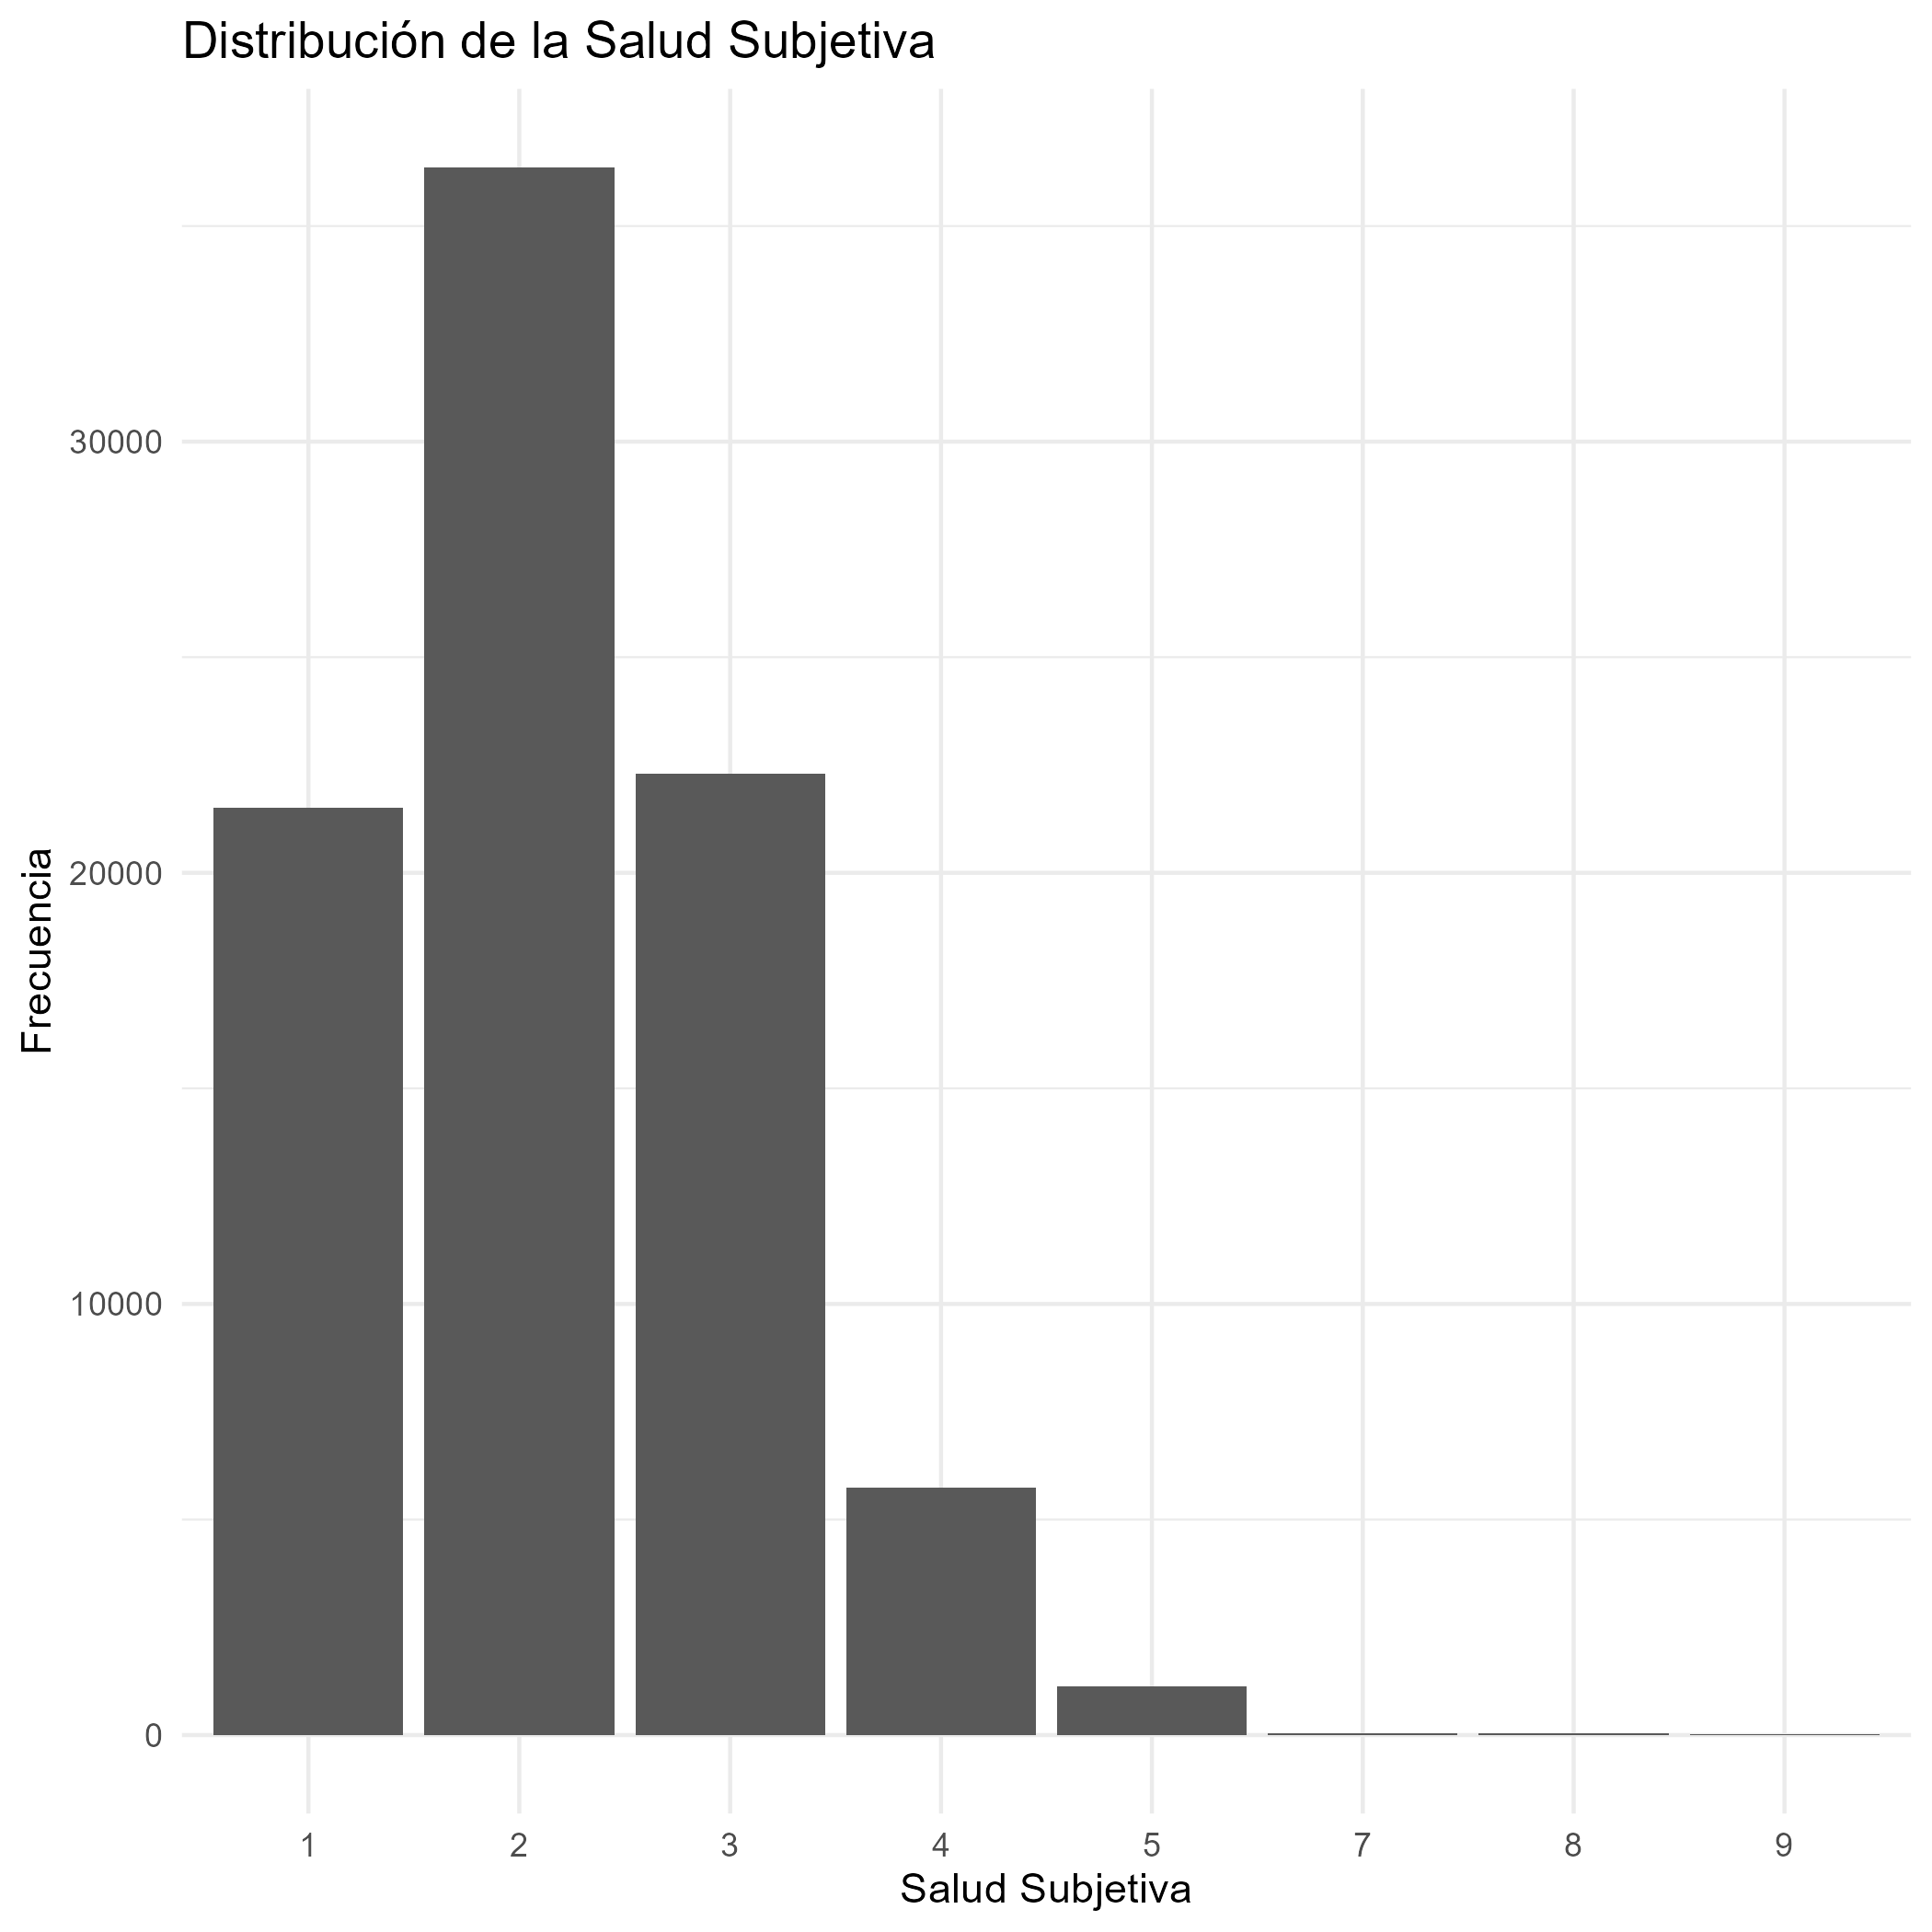
\includegraphics[width=0.8\textwidth]{C:/Users/User/Desktop/GITHUB/ProyectoCD---Modulo-8-Julio2024/INFORME/distribucion_salud_subjetiva.png}
\end{frame}
\begin{frame}
\frametitle{Gráfico}
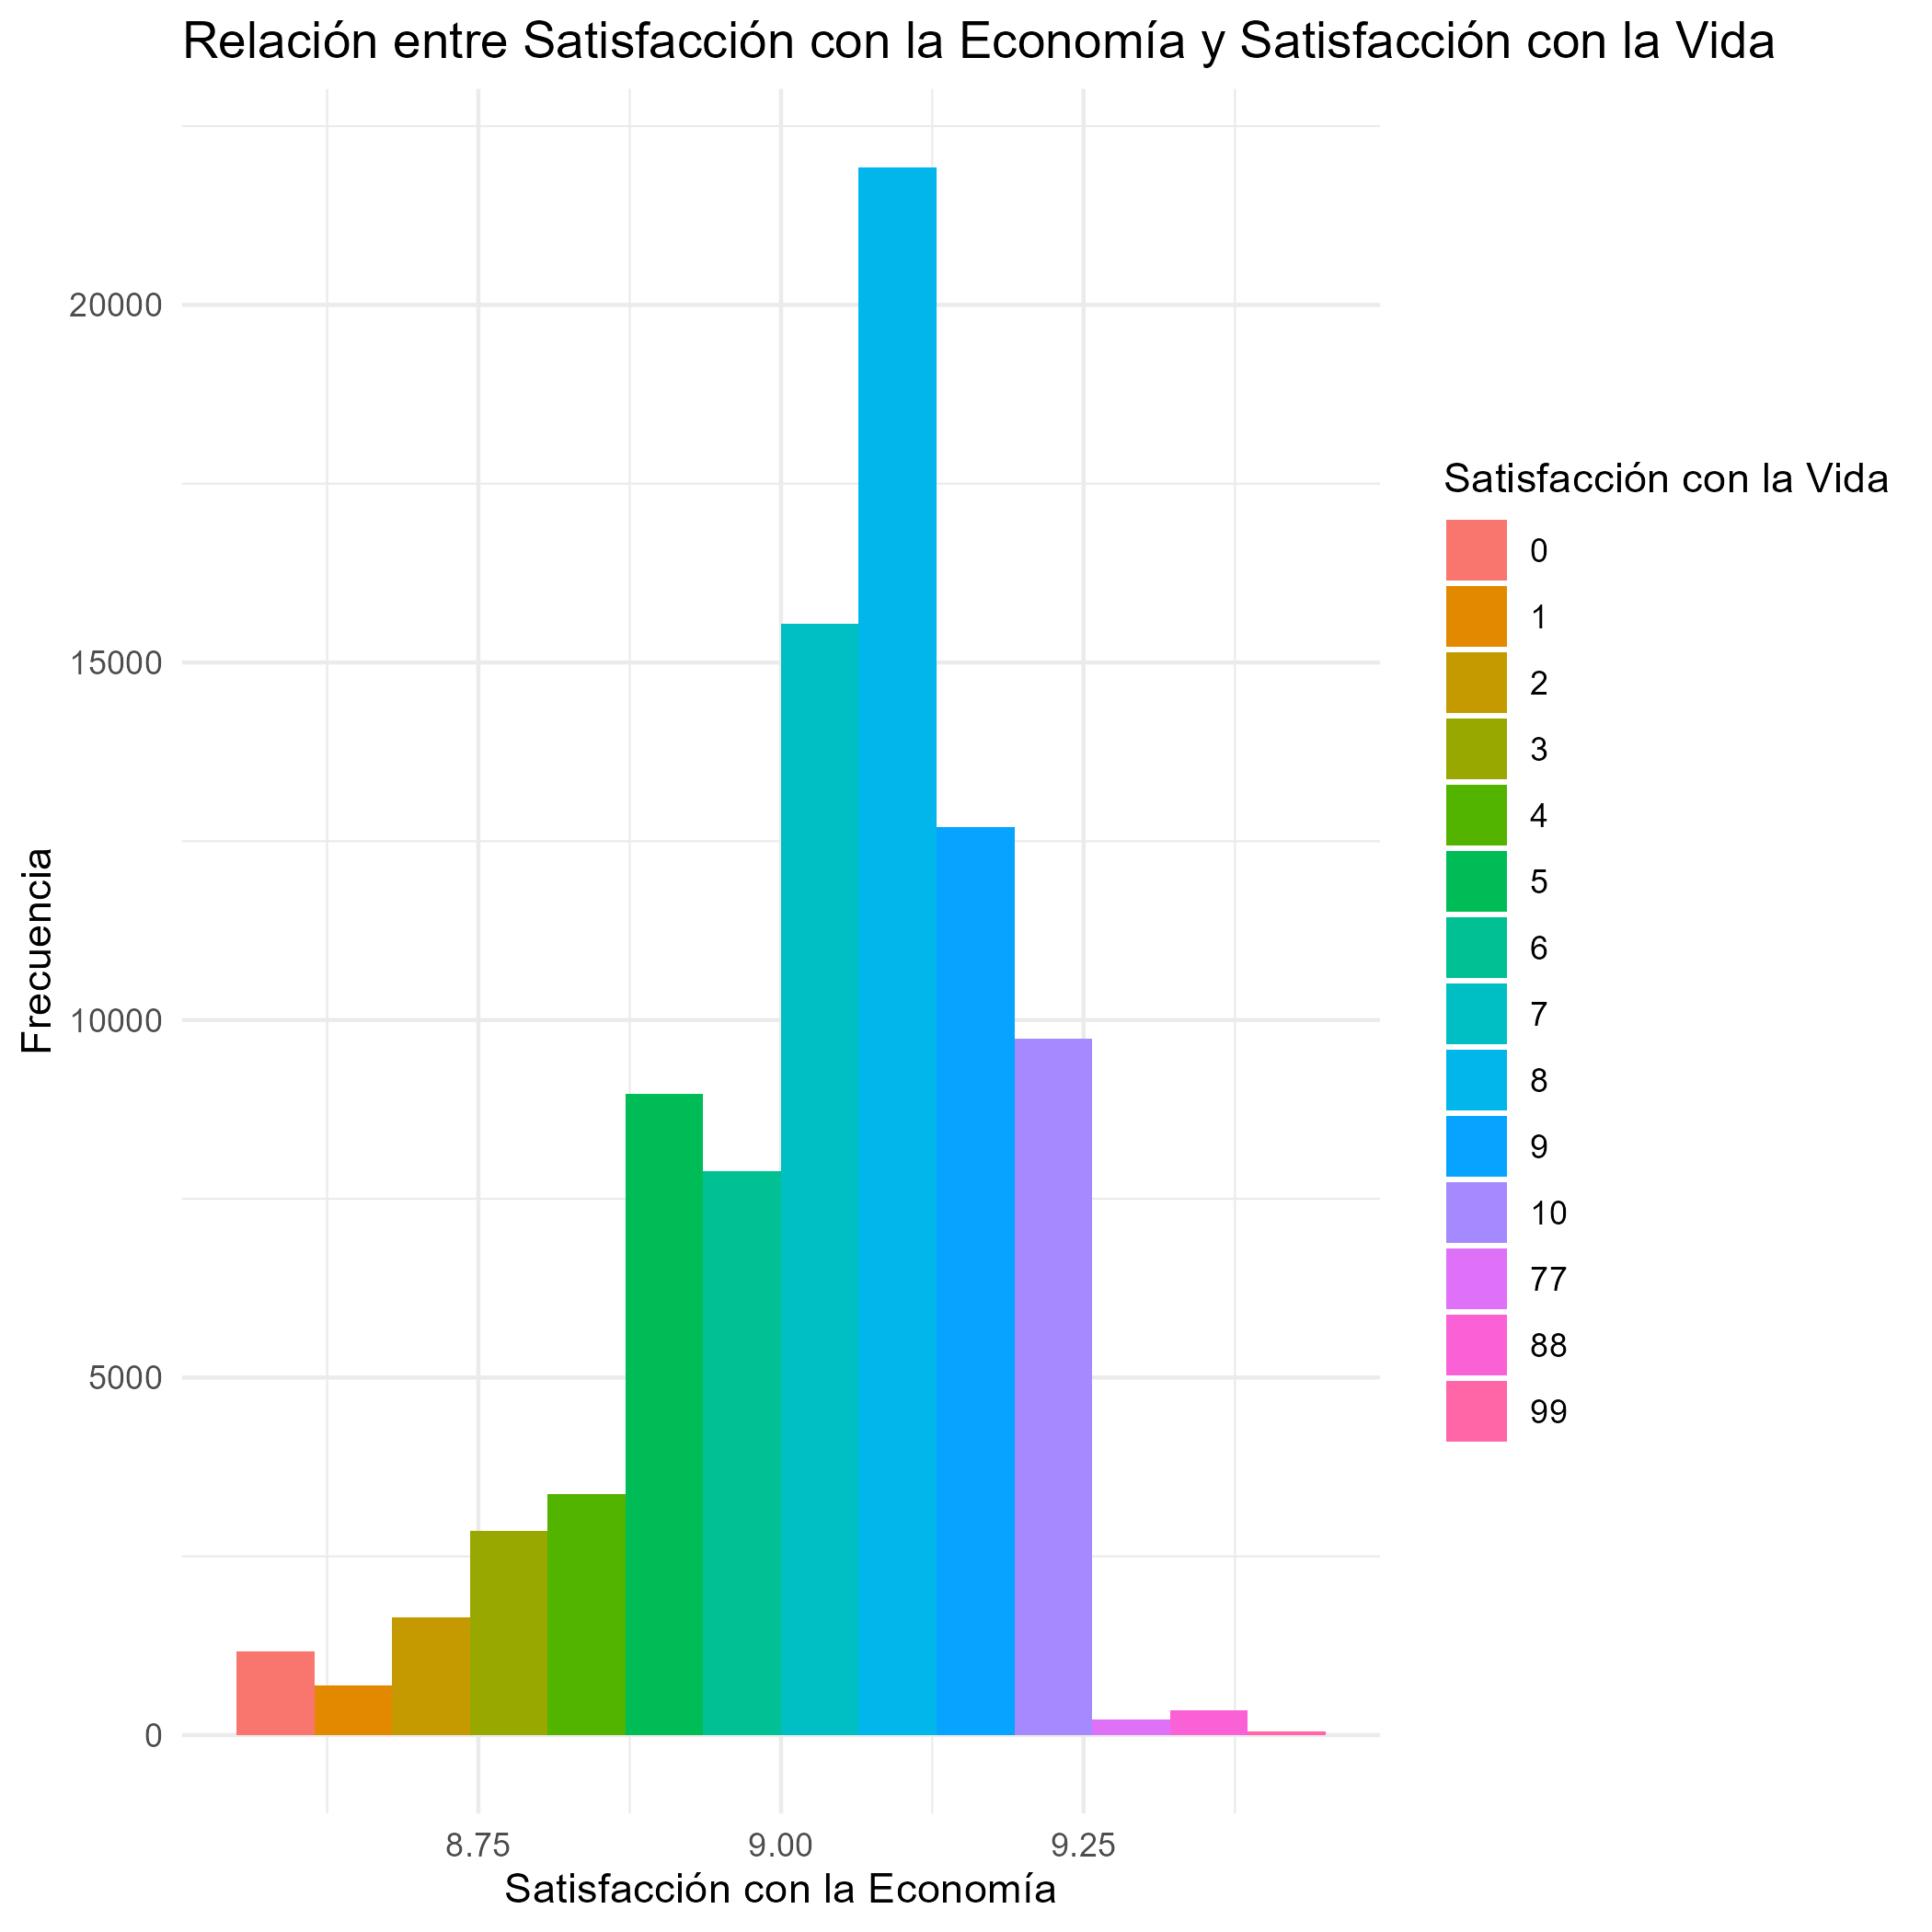
\includegraphics[width=0.8\textwidth]{C:/Users/User/Desktop/GITHUB/ProyectoCD---Modulo-8-Julio2024/INFORME/relacion_satisfaccion_vida_economia.png}
\end{frame}
\begin{frame}
\frametitle{Gráfico}
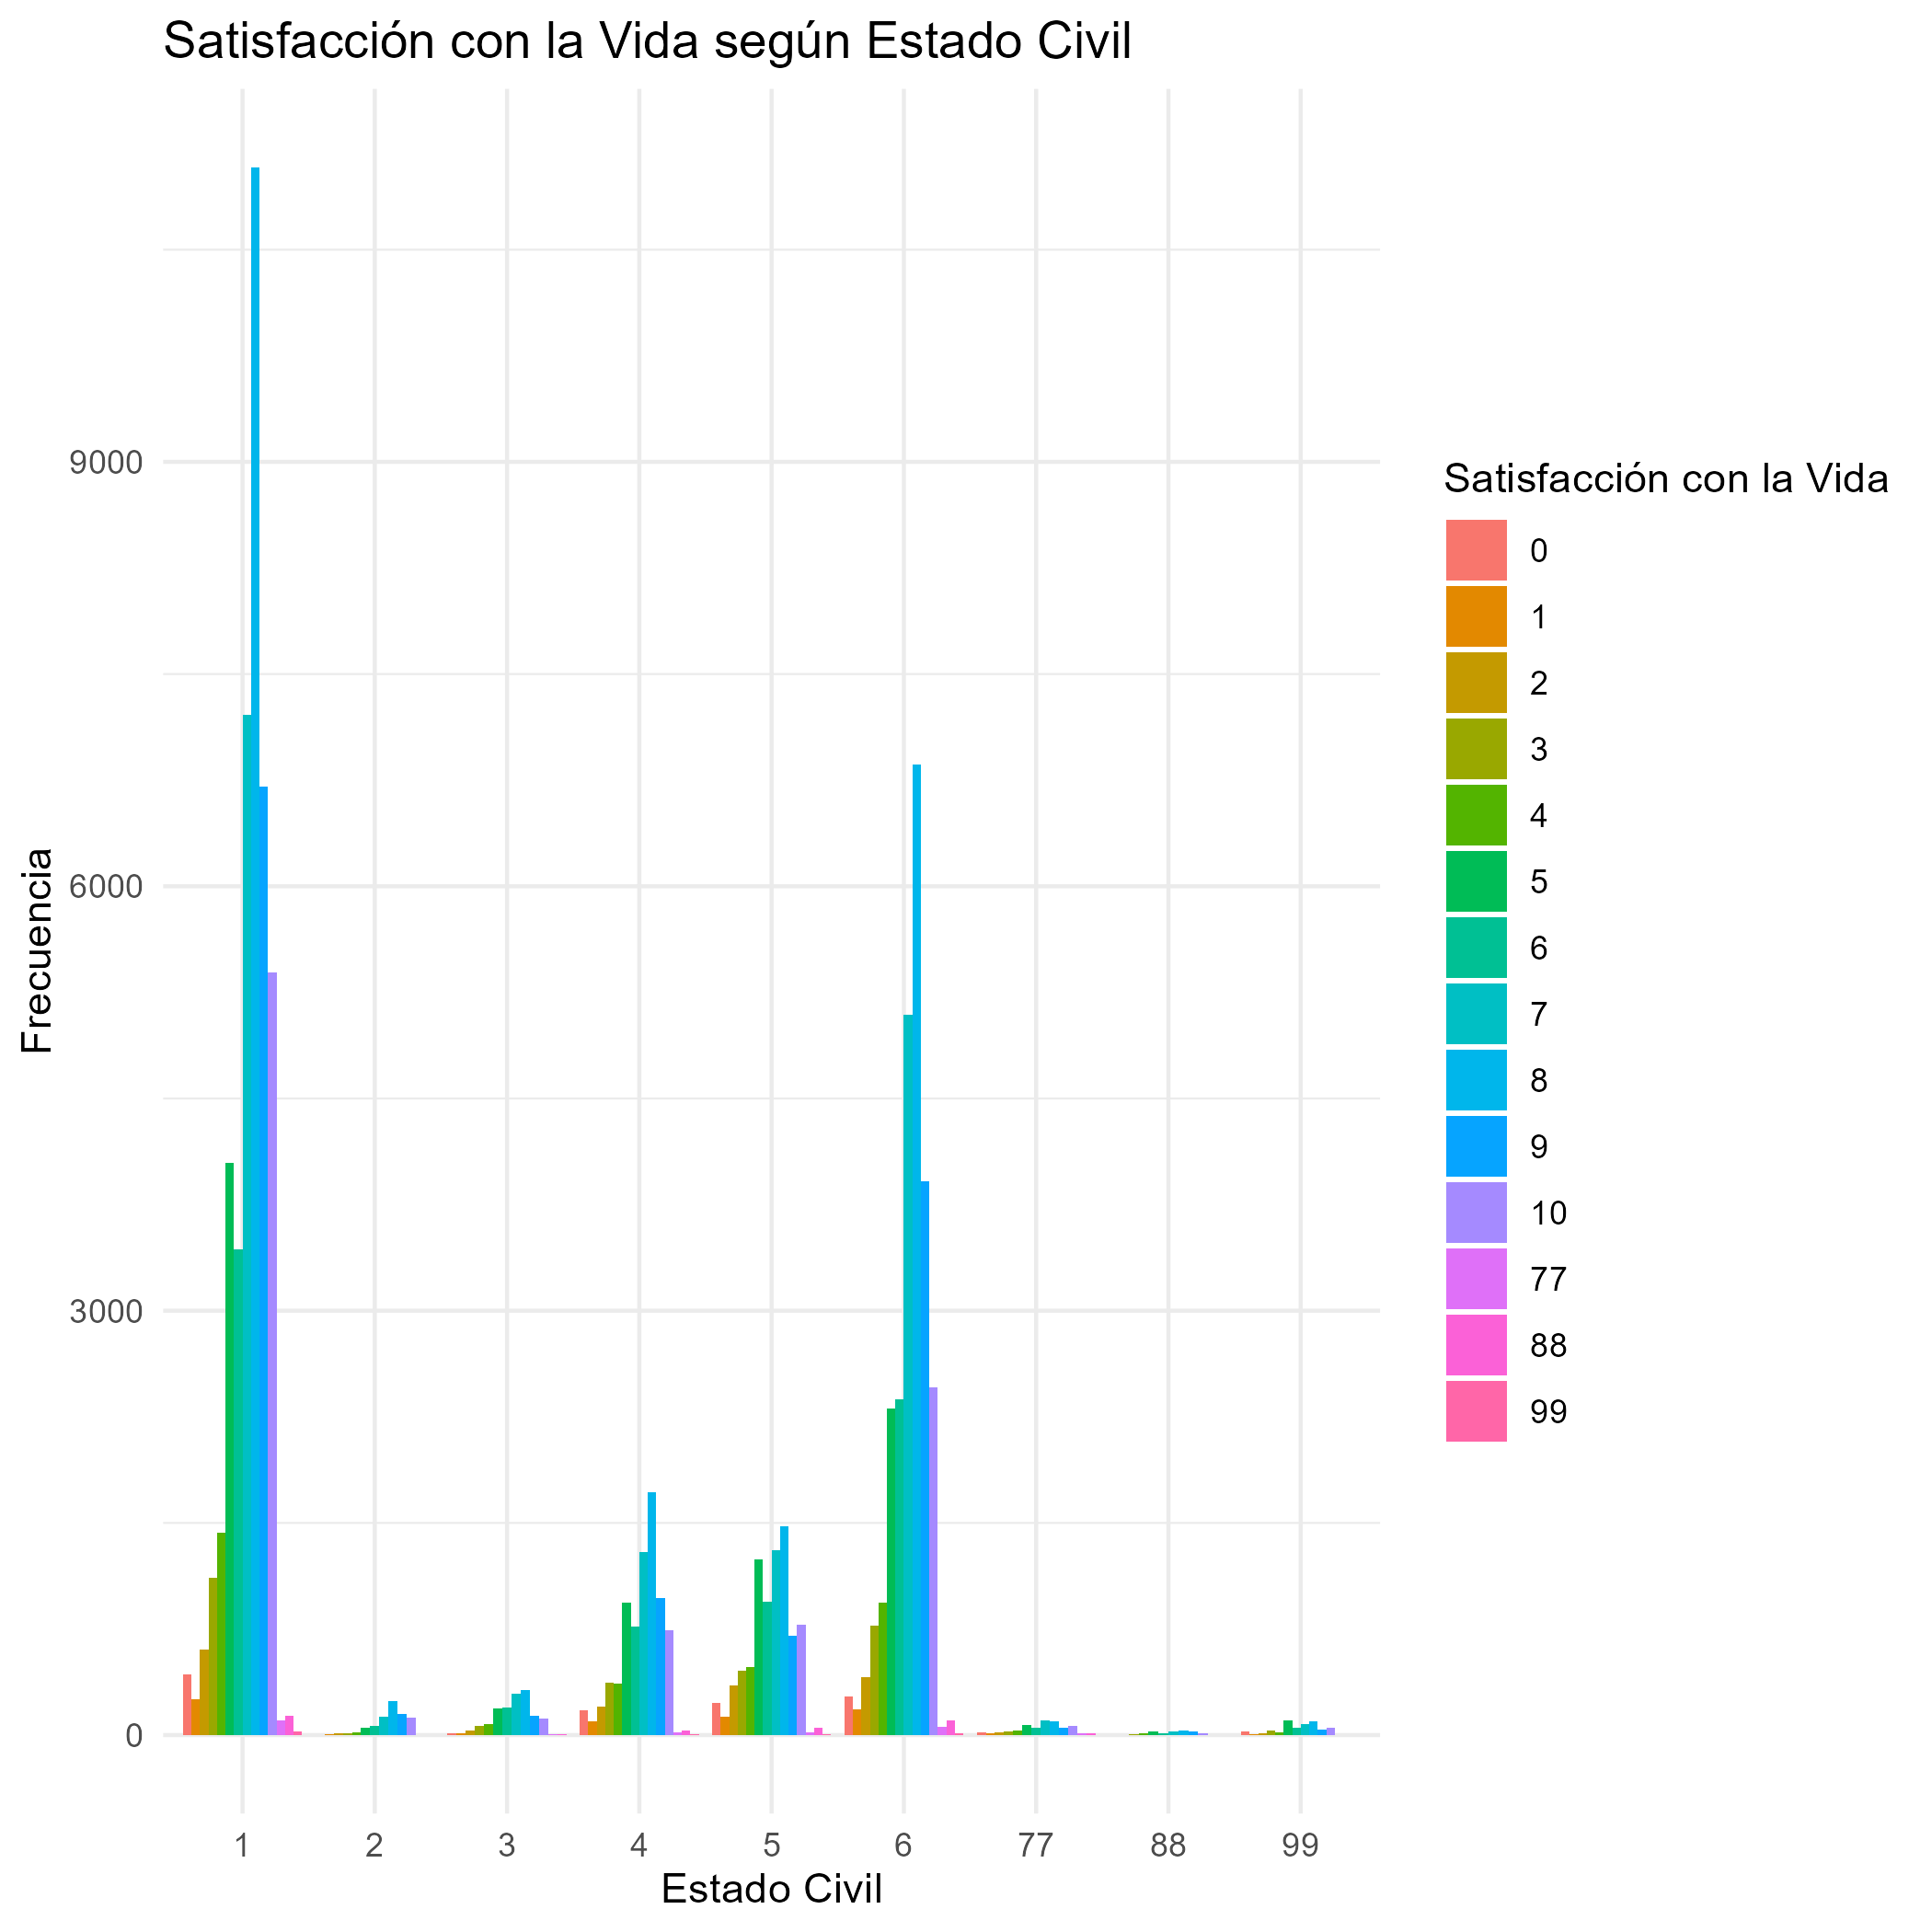
\includegraphics[width=0.8\textwidth]{C:/Users/User/Desktop/GITHUB/ProyectoCD---Modulo-8-Julio2024/INFORME/satisfaccion_vida_estado_civil.png}
\end{frame}
\begin{frame}
\frametitle{Gráfico}
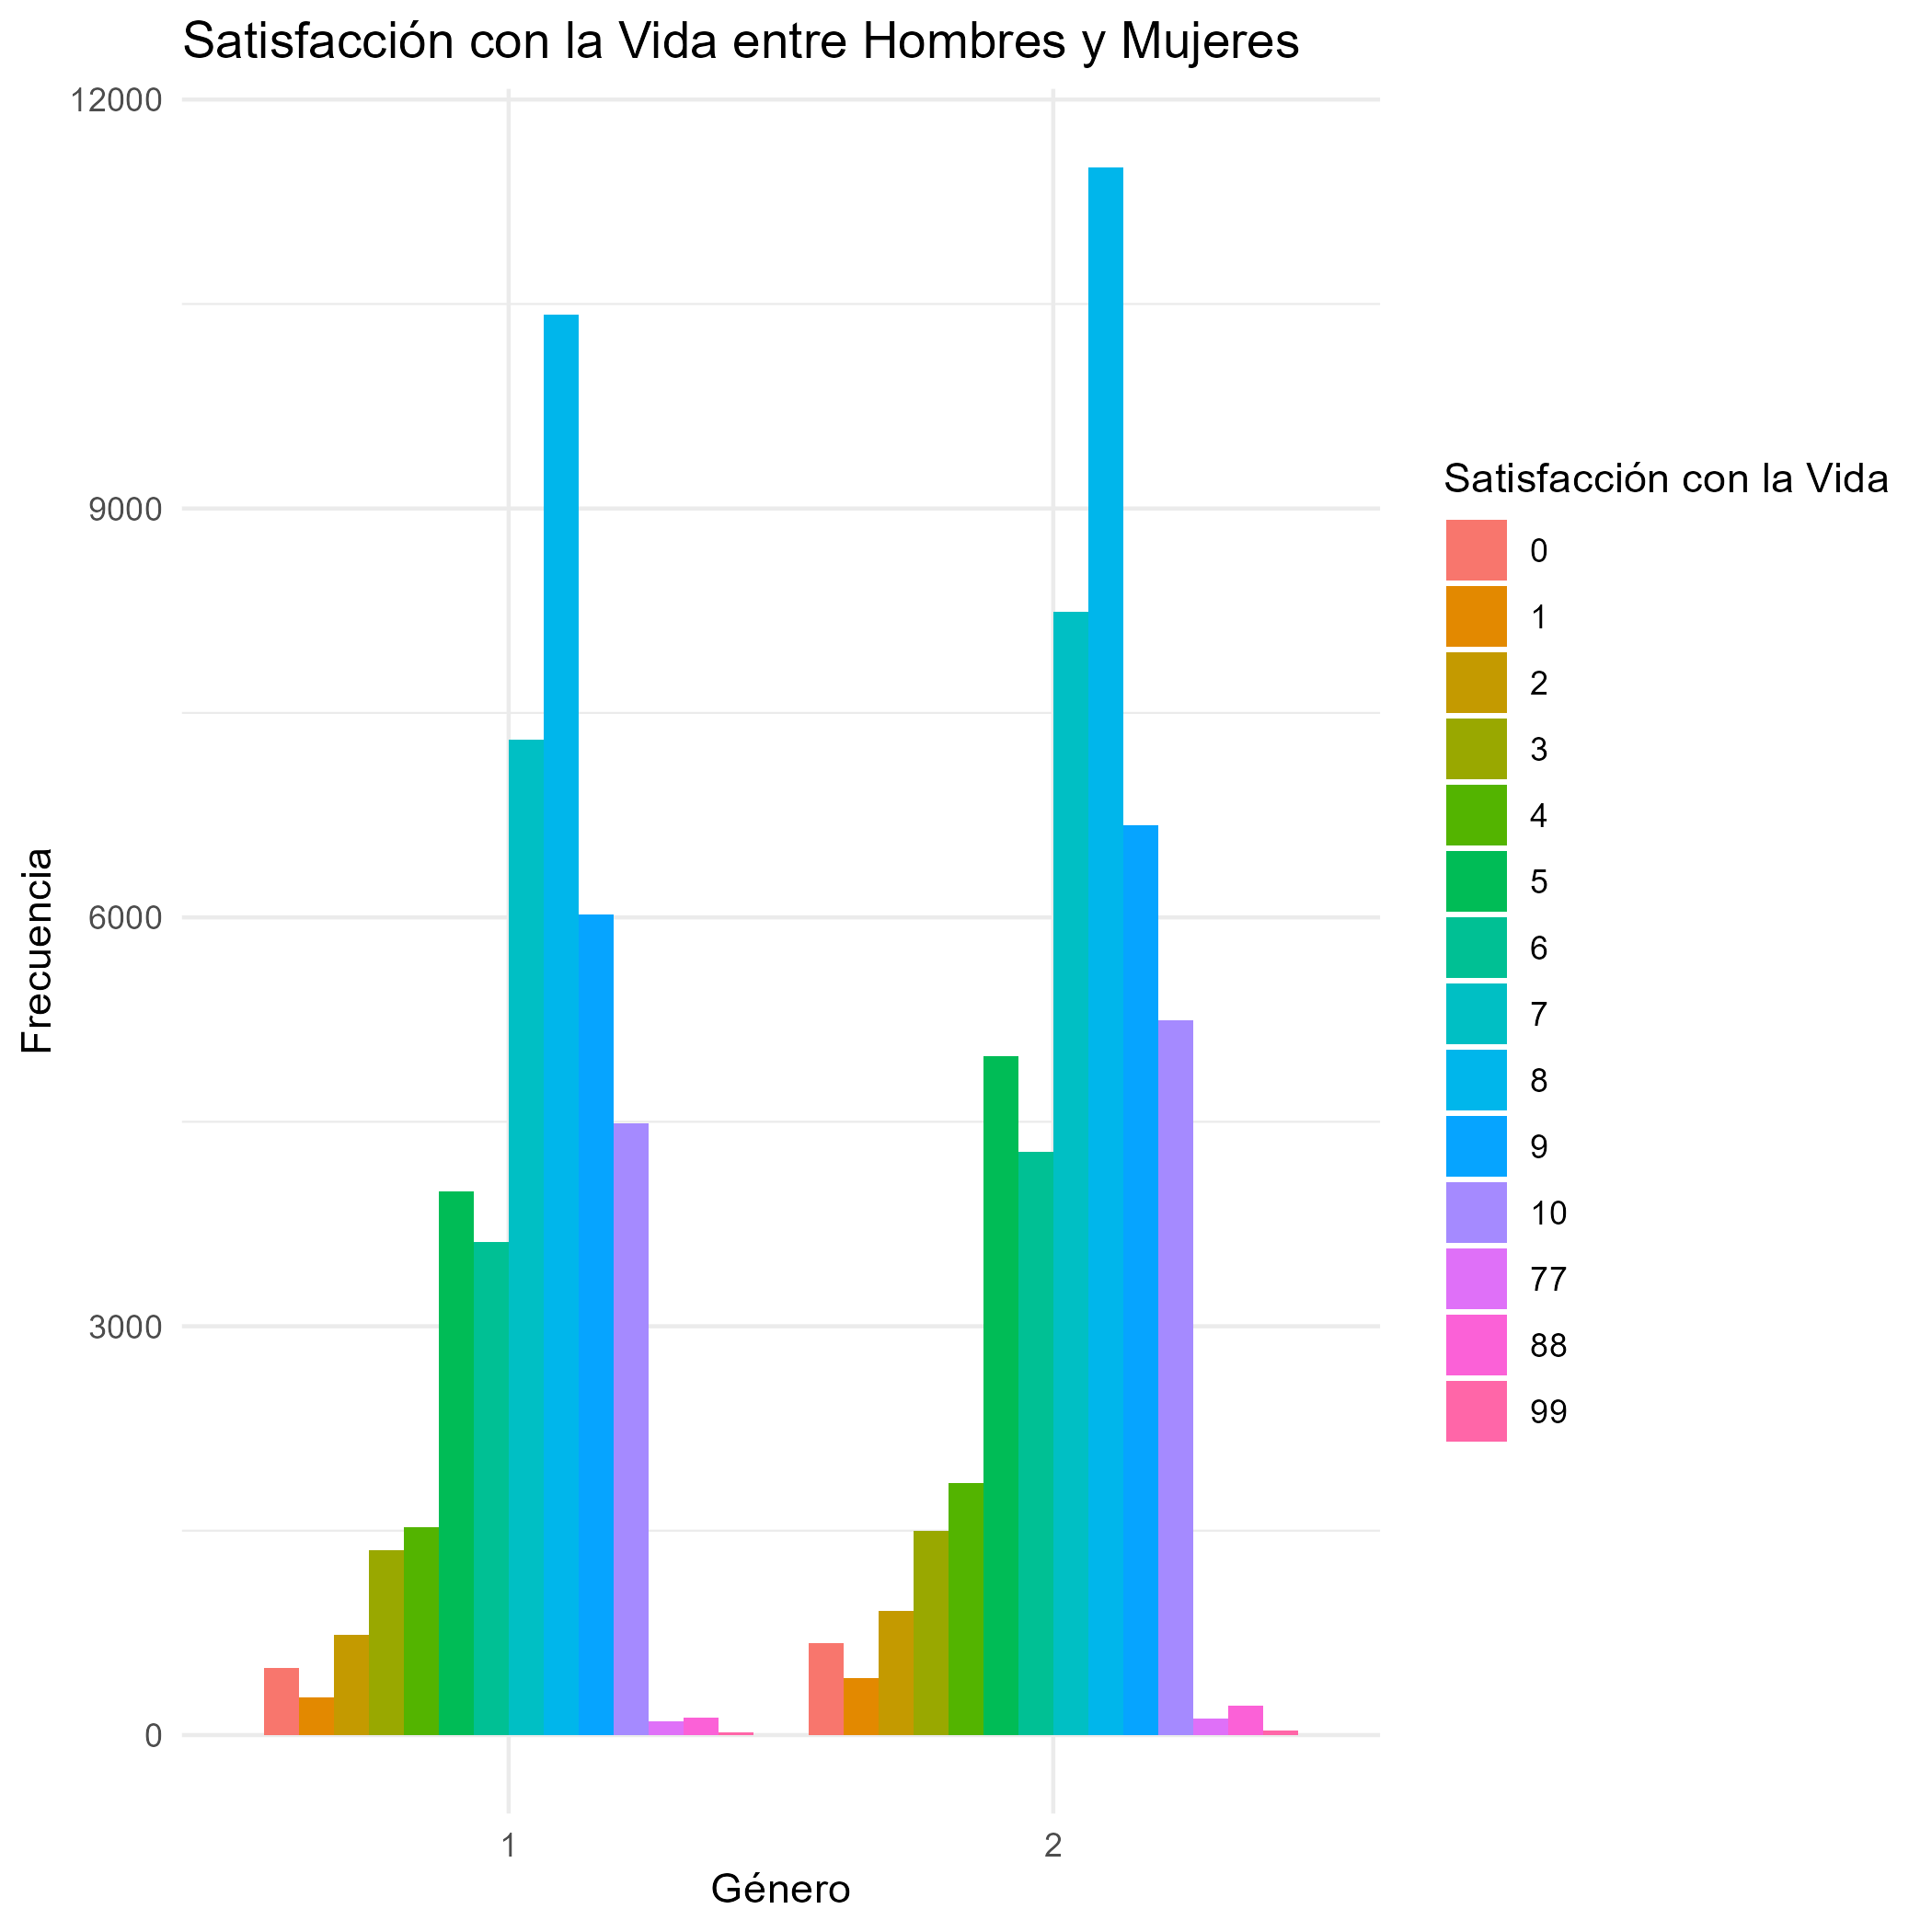
\includegraphics[width=0.8\textwidth]{C:/Users/User/Desktop/GITHUB/ProyectoCD---Modulo-8-Julio2024/INFORME/satisfaccion_vida_genero.png}
\end{frame}
\begin{frame}
\frametitle{Gráfico}
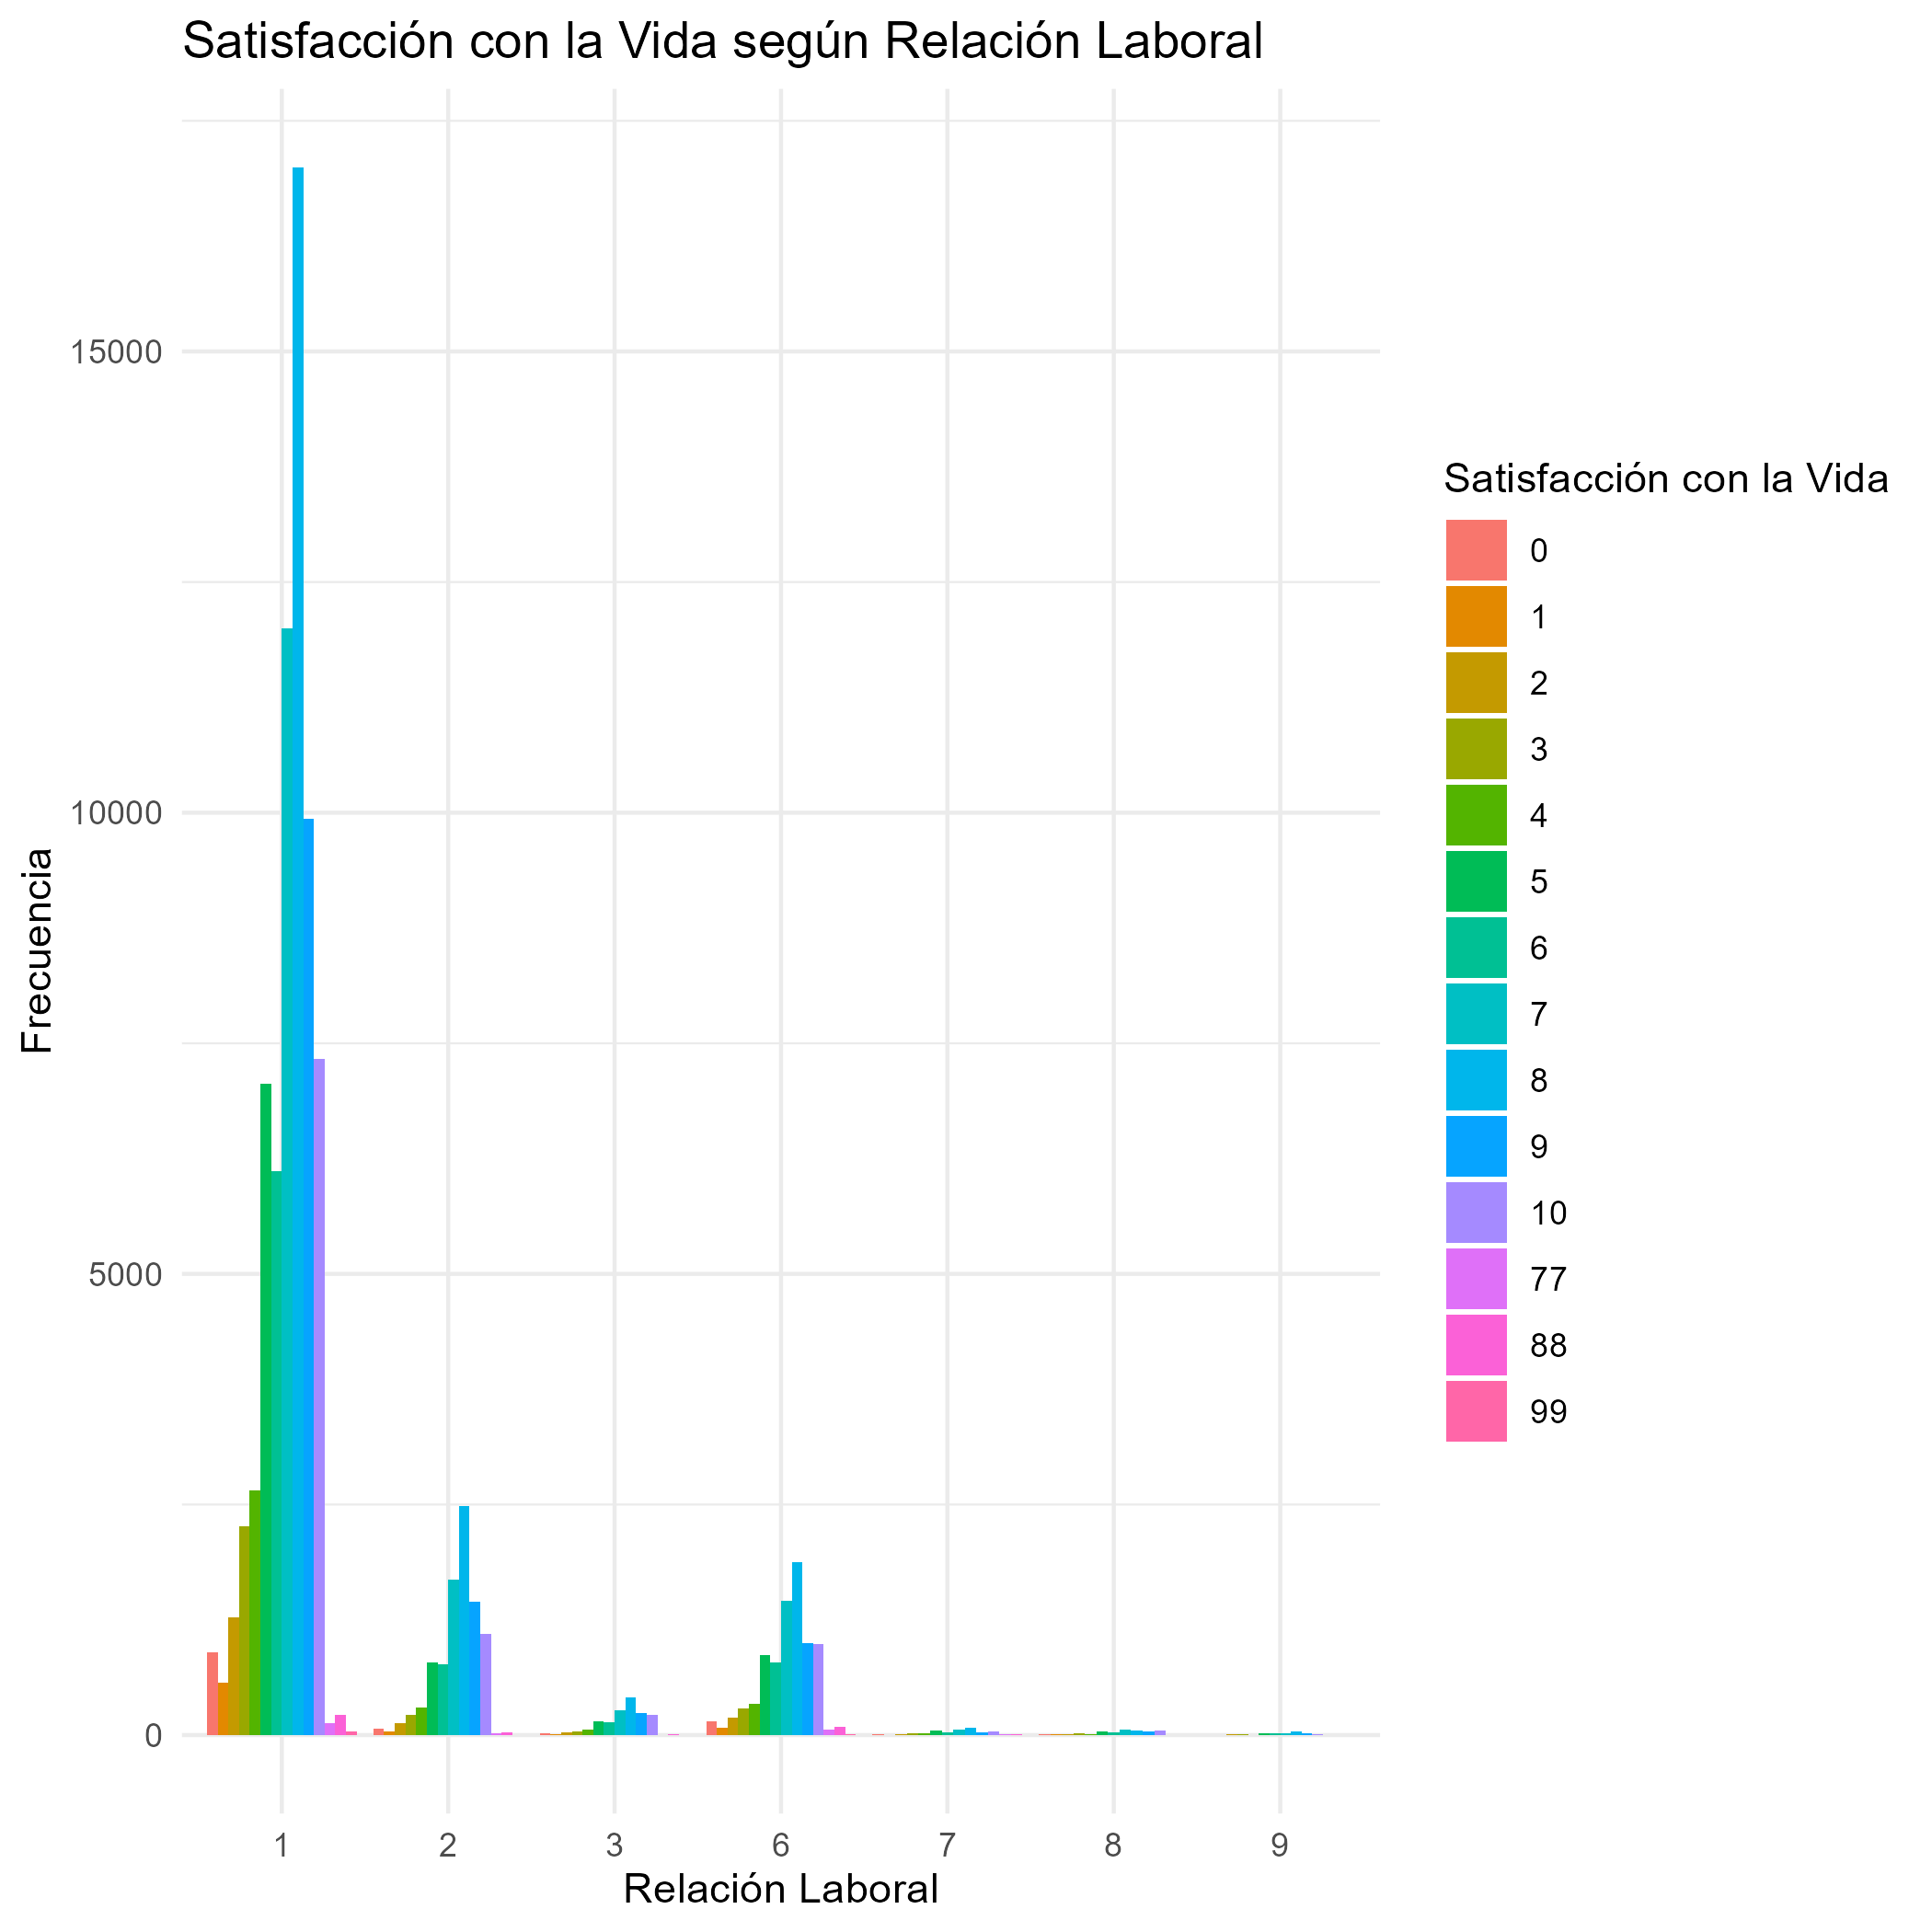
\includegraphics[width=0.8\textwidth]{C:/Users/User/Desktop/GITHUB/ProyectoCD---Modulo-8-Julio2024/INFORME/satisfaccion_vida_relacion_laboral.png}
\end{frame}


\section{Estadísticas Descriptivas}
\begin{frame}
  \frametitle{Estadísticas Descriptivas}
  La media de la edad de los encuestados es \textbf{\emph{56.5660852}} años, con una desviación estándar de \textbf{\emph{74.9179991}} años. La tabla siguiente muestra un resumen de las estadísticas descriptivas.
\end{frame}

\begin{kframe}


{\ttfamily\noindent\itshape\color{messagecolor}{\#\# Rows: 1 Columns: 6\\\#\# -- Column specification --------------------------------------------------------\\\#\# Delimiter: "{},"{}\\\#\# dbl (6): Edad\_Media, Edad\_SD, Satisfaccion\_Vida\_Media, Satisfaccion\_Vida\_SD,...\\\#\# \\\#\# i Use `spec()` to retrieve the full column specification for this data.\\\#\# i Specify the column types or set `show\_col\_types = FALSE` to quiet this message.}}\end{kframe}\begin{table}

\caption{\label{tab:table_chunk}Tabla de Estadísticas Descriptivas}
\centering
\begin{tabular}[t]{r|r|r|r|r|r}
\hline
Edad\_Media & Edad\_SD & Satisfaccion\_Vida\_Media & Satisfaccion\_Vida\_SD & Felicidad\_Media & Felicidad\_SD\\
\hline
56.56609 & 74.918 & 8.131769 & 2.185627 & 8.357512 & 1.949245\\
\hline
\end{tabular}
\end{table}



\end{document}

